% Emacs, this is -*-latex-*-
\documentclass[main.tex]{subfiles}

\begin{document}
\section{Gamma Ray Astrophysics}
Gamma ray astrophysics studies the physics and the sources of particles at high energies (E >$1$ GeV). While astronomy is a centuries-old science, gamma-ray astrophysics has only come into play since the advent of satellite technology and subsequently of Imaging Atmospheric Cherenkov Telescopes (IACTs) in the 1980s. Due to constraints from atmospheric interactions, direct detection of high energy emissions is not feasible with traditional ground-based instruments. However satellites are able to circumvent these issues, and IACTs are able to use them to their benefit.\par

High-energy (HE, E >$1$ GeV) or very high energy (VHE, E >$100$ GeV) gamma-ray emission is a signature of extreme astrophysical processes like relativistic jets and strong electromagnetic fields. These processes are among the most energetic phenomena in the universe and are present in active galactic nuclei (AGN), pulsar wind nebulae (PWN), and pulsars. Since the penetration depth for higher energy photons in the atmosphere is shorter than their optical counterparts, they become much harder to manipulate using conventional methods like those used for photons. Instead, methods of high-energy particle physics and detector technology used for other high-energy particles are used for gamma-ray detection. Satellite-based instruments like the Fermi Large Area Telescope (LAT) are able to detect lower-energy gamma rays (30 MeV -- 100 GeV) directly through tracking pair production $e^+/e^-$ pairs, but for very high energy (VHE) gamma rays (E$> 100$ GeV) the much lower photon flux means that effective areas required for significant statistics are much larger, and not feasible for satellite-based instruments.
\subsection{Ground Based Gamma-Ray Astrophysics}
The Whipple Collaboration pioneered the technique for indirect detection of gamma rays through the collection of Cherenkov photons emitted from extensive air showers generated from high-energy photon interactions with the atmosphere. The direction of the primary photons can be determined by imaging the air showers with telescopes. This also enables the rejection of hadronic showers from cosmic rays and provides an effective area much larger than is possible with space-based instruments. Cherenkov light used to detect these showers arrives in a region with a radius of $\sim 100$ m. The current generation of IACTs uses multiple telescopes which provide better sensitivity, better hadronic rejection and larger effective areas than individual telescopes\cite{Park:2017uxb}. In the thirty years of ground-based gamma ray astrophysics, over 200 VHE sources have been detected. \par
The current generation of ground based gamma-ray observatories includes three major telescope arrays. The MAGIC array, located on the Canary Islands of La Palma, Spain consists of two IACTs with 17 m diameter reflectors. The H.E.S.S. array in the Khomas Highlands of Namibia, is an array of five IACTs, four of which have 13 m diameter reflectors while the fifth, in the center of the array has a 28 m reflector. The VERITAS array in Arizona, US, the subject of this thesis, is an array of four telescopes, each with reflectors 12 m in diameter.
\section{VERITAS Overview}
The Very Energetic Radiation Imaging Telescope Array System (VERITAS) is an array of four IACTs at the Fred Lawrence Whipple Observatory in southern Arizona, which started operating in 2007. Gamma rays are detected through imaging Cherenkov radiation emitted from relativistic charged particles (primarily $e^+/e^-$) in air showers initiated by VHE gamma rays. This section contains a brief description of the instrument and the technique used in this experiment. After the moving of one telescope in 2009, and upgrading the camera to higher quantum efficiency photo-multiplier tubes (PMTs) in 2012, VERITAS is sensitive to an energy range between $\sim85$GeV and $\sim30$TeV and has a field of view of $3.5^\circ$.
\begin{figure}[htbp]
  \centering
  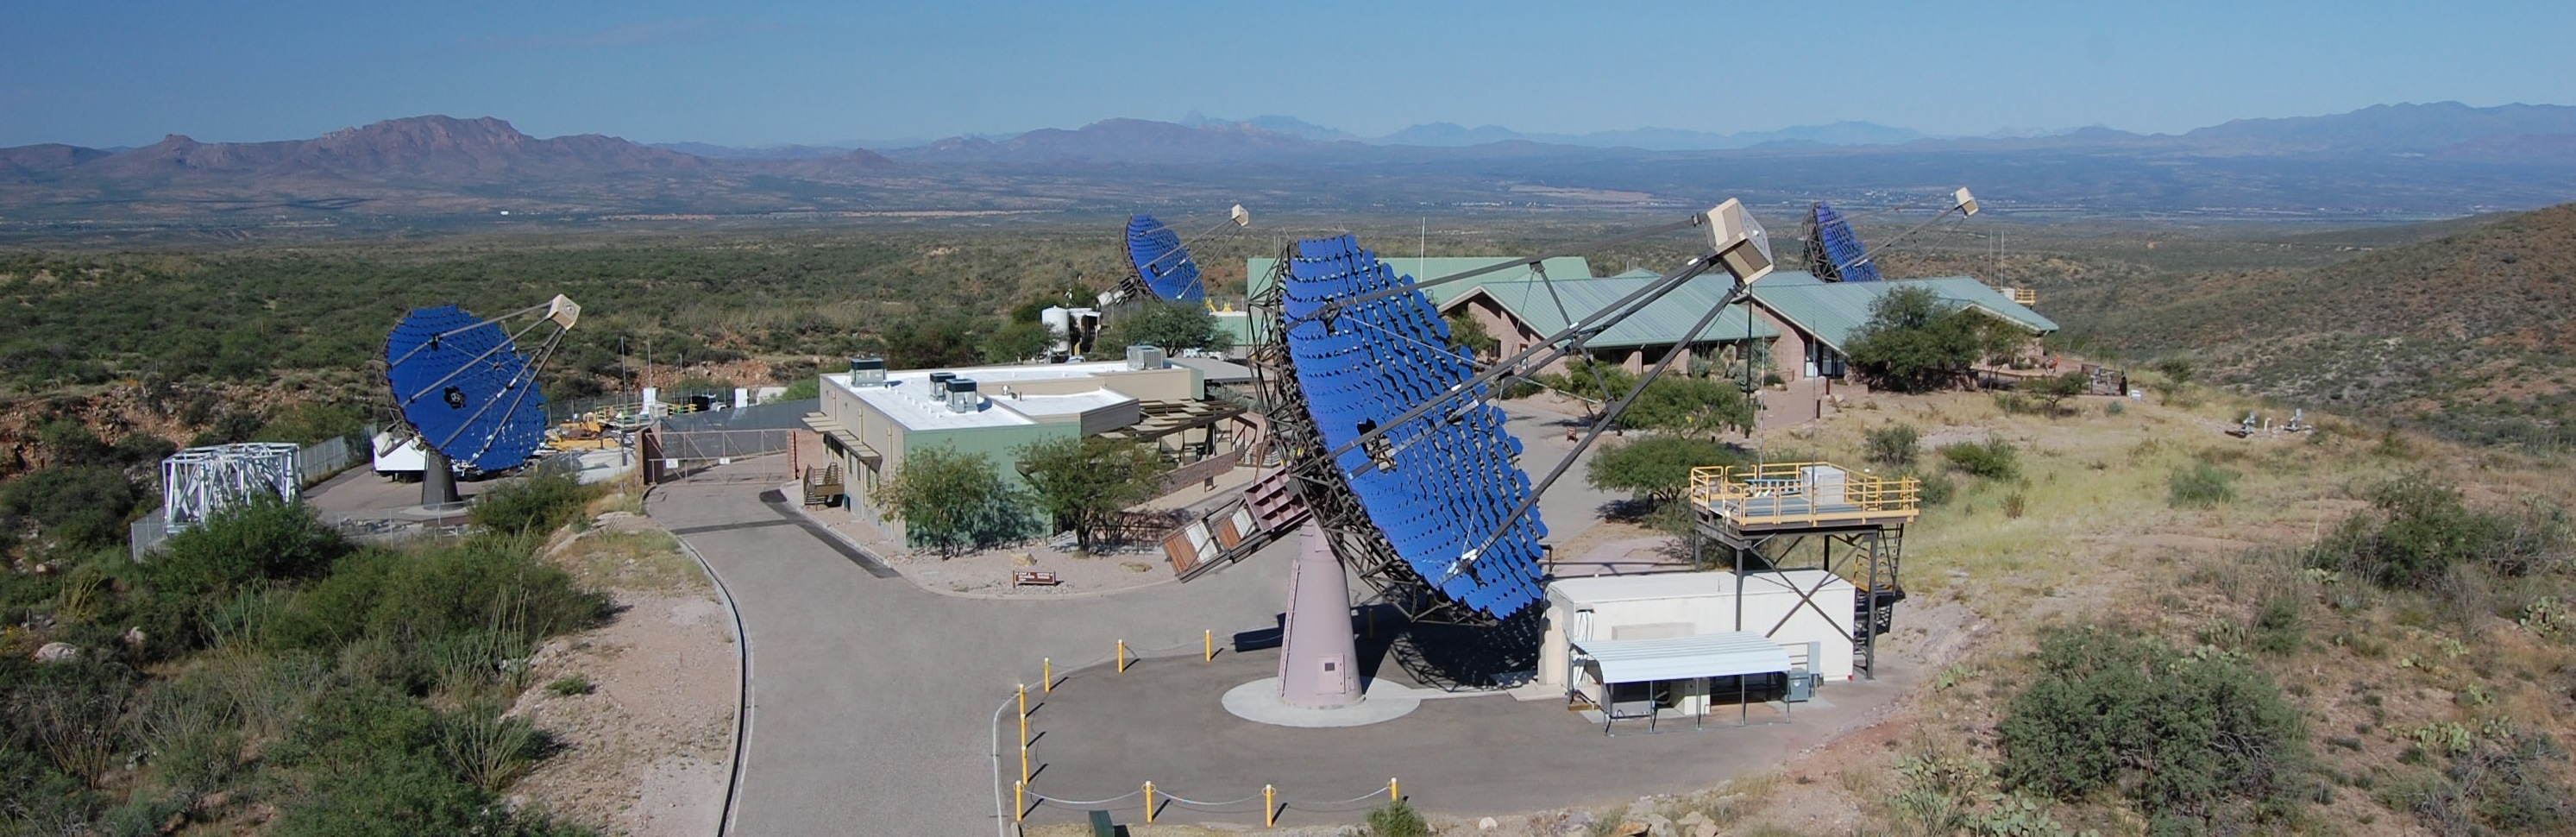
\includegraphics[width=\linewidth]{images/veritas_standard}
  \caption[Photograph of the VERITAS telescopes and the control center.]{Photograph of the VERITAS telescopes and the control center. Photo taken from \cite{veritas_web}.}
  \label{veritas_standard}
\end{figure}

\subsection{Gamma-Ray Initiated Extensive Air Showers}
\label{Gamma-ray-EAS}
At gamma-ray energies, photons interact with the upper atmosphere resulting primarily in pair production of $e^+/e^-$ pairs as shown in Fig. \ref{fig:EAS_img}. On propagating through the atmosphere, electrons/positrons undergo ``bremsstrahlung'' and emit gamma rays. ``Bremsstrahlung'', German for ``breaking radiation'', is a process where a charged particle (in this case an electron/positron) accelerated in the electromagnetic field of a nucleus loses energy by emitting photons. The bremsstrahlung photons can again undergo pair production and the shower continues as before resulting in an exponentially growing number of particles, with a decreasing mean particle energy. \par
Higher energy particles are beamed more strongly forward and so in the VHE gamma-ray energy scale, the particle shower has a small footprint ($\sim 30$ m) transverse to the direction of the initiating particle, and a large longitudinal distribution ($\sim10$ km). As the shower proceeds, the mean energy of the particles gets progressively smaller, due partly to division among a larger number of particles and partly due to loss to ionization. Eventually, the process reaches an energy where Compton scattering becomes the dominant process causing energy loss, and the cascade stops. At this point, the shower energy dissipates into the atmosphere through ionization. Since the cascade which was so far growing exponentially halts here, the number of particles does not increase beyond this point and this point is referred to as the shower-maximum.
\begin{figure}[htbp]
  \centering
  \subfigure{ 
    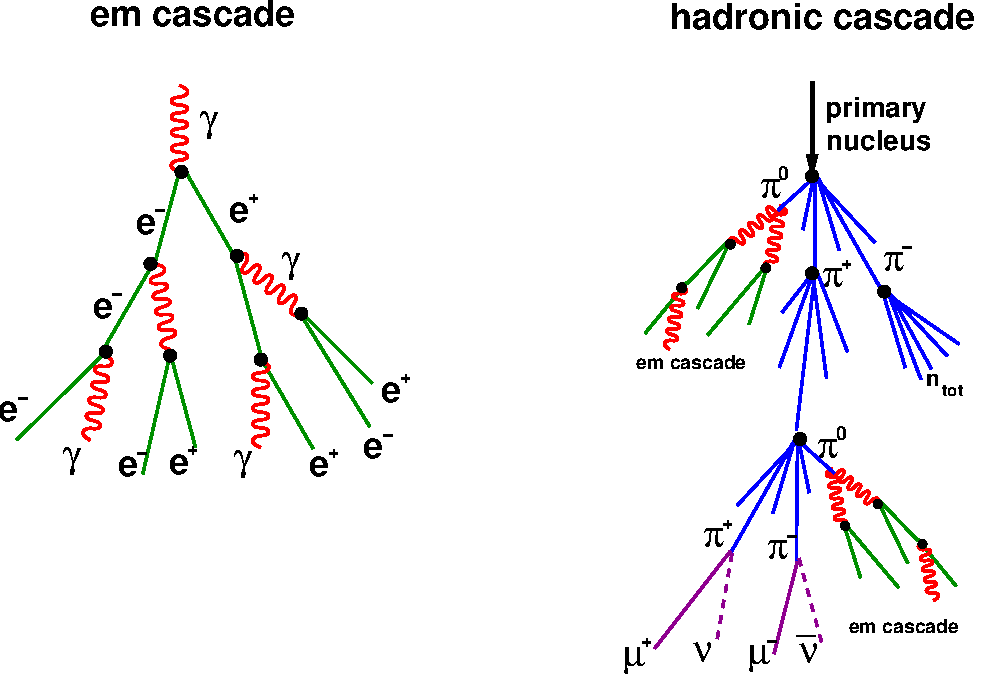
\includegraphics[width=0.68\linewidth]{images/gamma_hadron_illustration}
    % \label{fig:gamma_hadron_shower}
  }
  % \subfigure{
  %   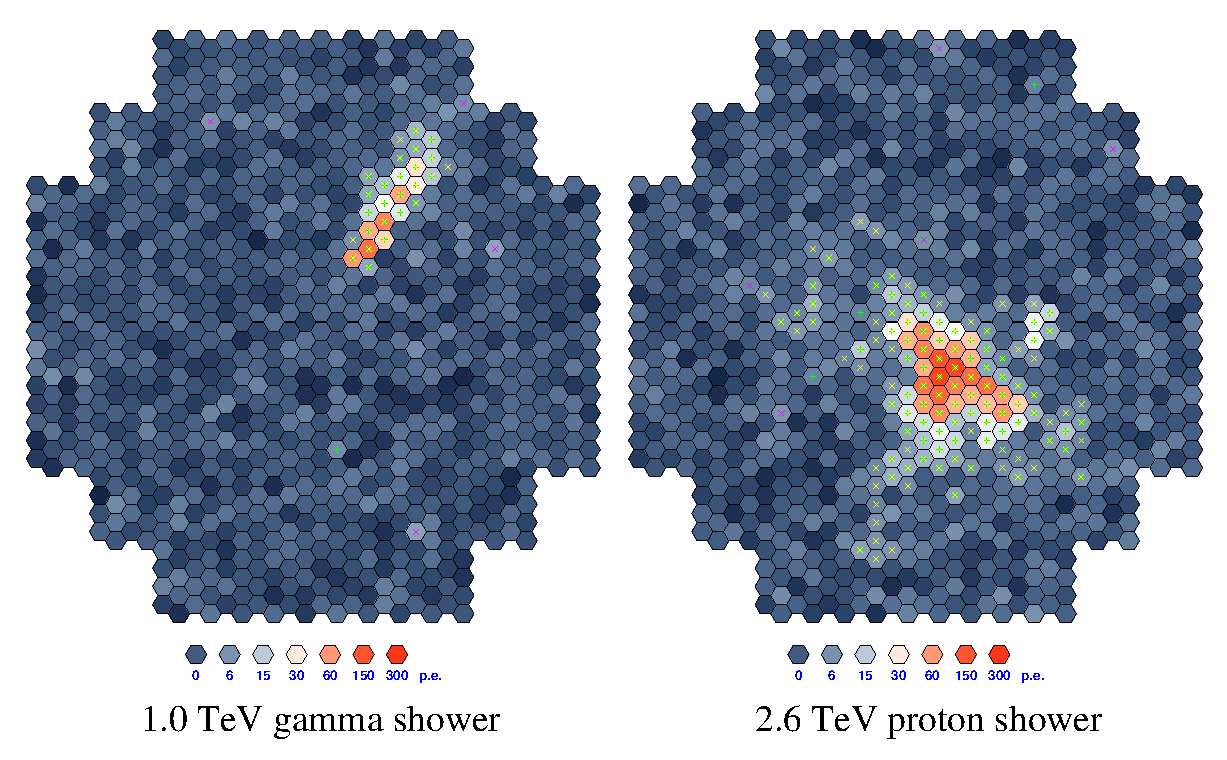
\includegraphics[width=0.68\linewidth]{images/gamma_hadron_sep}
  %   \label{fig:gamma_hadron_face}
  %   Camera face showing the difference between photons and hadron images (bottom) \cite{Gamma_Hadron_Sep}
  % }
  \caption[Processes involved in generating extensive air showers.]{Processes involved in generating extensive air showers \cite{EAS_2018}.}
  \label{fig:EAS_img}
\end{figure}
\subsection{Cherenkov Radiation}
Cherenkov radiation is electromagnetic radiation emitted by a dielectric medium when a charged particle travels through it at a speed faster than the speed of light in the medium. The mechanism is commonly described as the analog of a sonic boom and the resulting shock wave front. Cherenkov radiation, when intense, appears as a bluish glow like that noticed in the pools of water shielding some nuclear reactors. The phenomenon was experimentally studied by the Soviet physicist Pavel A. Cherenkov in 1934 and was explained by Ilya M. Frank and Igor Y. Tamm in 1937.\par

\begin{figure}[htbp]
  \centering
  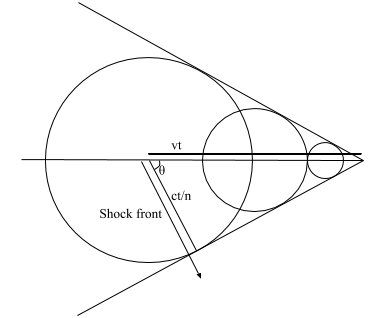
\includegraphics[width=0.6\linewidth]{images/Cherenkov}
  \caption[Mechanism of Cherenkov radiation.]{Mechanism of Cherenkov radiation.}
  \label{fig:Cherenkov}
\end{figure}

The speed of light in a medium is given by $c/n$ where $n$ is the refractive index of light in the medium. When the speed of the particle exceeds this speed ($v>c/n$), a shock front appears between the region where an electric field due to the charged particle is present and one where it is not because the electric field can only propagate at the speed of light in the medium ($c/n$). The shock front travels at an angle given by $\theta = \cos^{-1}(c/vn) = \cos^{-1}(1/\beta n)$ with radiation emitted in a cone with angle $\theta$ from the direction of propagation of the initiating charged particle as shown in Fig. ~\ref{fig:Cherenkov}. The number of photons per unit length of particle path per unit of wavelength is given by 
\begin{equation}
  \frac{d^2N}{dxd\lambda} = \frac{4\pi^2z^2e^2}{hc\lambda}\left(1-\frac{1}{n^2\beta^2}\right) = \frac{2\pi z^2}{\lambda^2}\alpha\sin^2\theta_C
\end{equation}
The inverse dependence on the wavelength means that the photons radiated are mostly on the low-wavelength end of the spectrum. Since Cherenkov radiation is a coherent process, the electric field is perpendicular to the surface of the emission cone and the emission is completely polarized.
\subsection{Imaging Atmospheric Cherenkov Telescopes}
Imaging atmospheric Cherenkov telescopes (IACTs) detect the light produced in an extensive air shower (EAS) by the primary particle. EAS emit a cone of forward-beamed Cherenkov photons with a half-opening angle of $\sim 1^\circ$ \cite{antonelli2009}. This beam illuminates an elliptical region on the ground called the light pool which has an area of the order of $10^5$ $\tx{m}^2$, with variations depending on the altitude of the shower maximum and inclination of the shower axis. \par
The Cherenkov technique resolves (in space and time) the shower development image captured by the telescope camera. This information is used to distinguish between different types of showers (hadronic vs $\gamma$-ray-initiated) by using the different spatial spread of the showers depending on initial particles. In particular, for VHE $\gamma$-ray showers, because the shower is compact in the transverse direction the direction of the ensuing shower is roughly along a cone with the thickness of the cone inversely dependent on the energy.% -- higher energy causes more beaming
 For hadronic showers, the initial interactions lead to a less compact spread in direction of the resulting particles.\par
\begin{figure}[htbp]
  \centering
  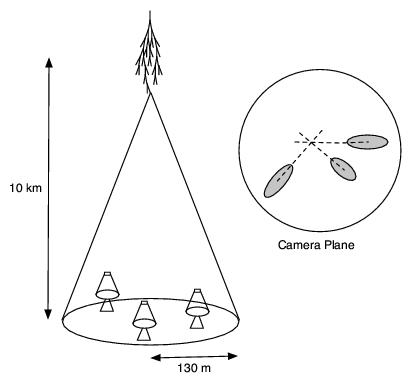
\includegraphics[width=0.68\linewidth]{images/IACT}
  \caption[Illustration of an IACT array.]{Illustration of an IACT array, with typical shower height and radius of light pool for $\gamma$-rays with primary energy $>100$ GeV. Picture taken from \cite{veritas_web}}
  \label{fig:IACT}
\end{figure}
\begin{figure}[htbp]
  \centering
  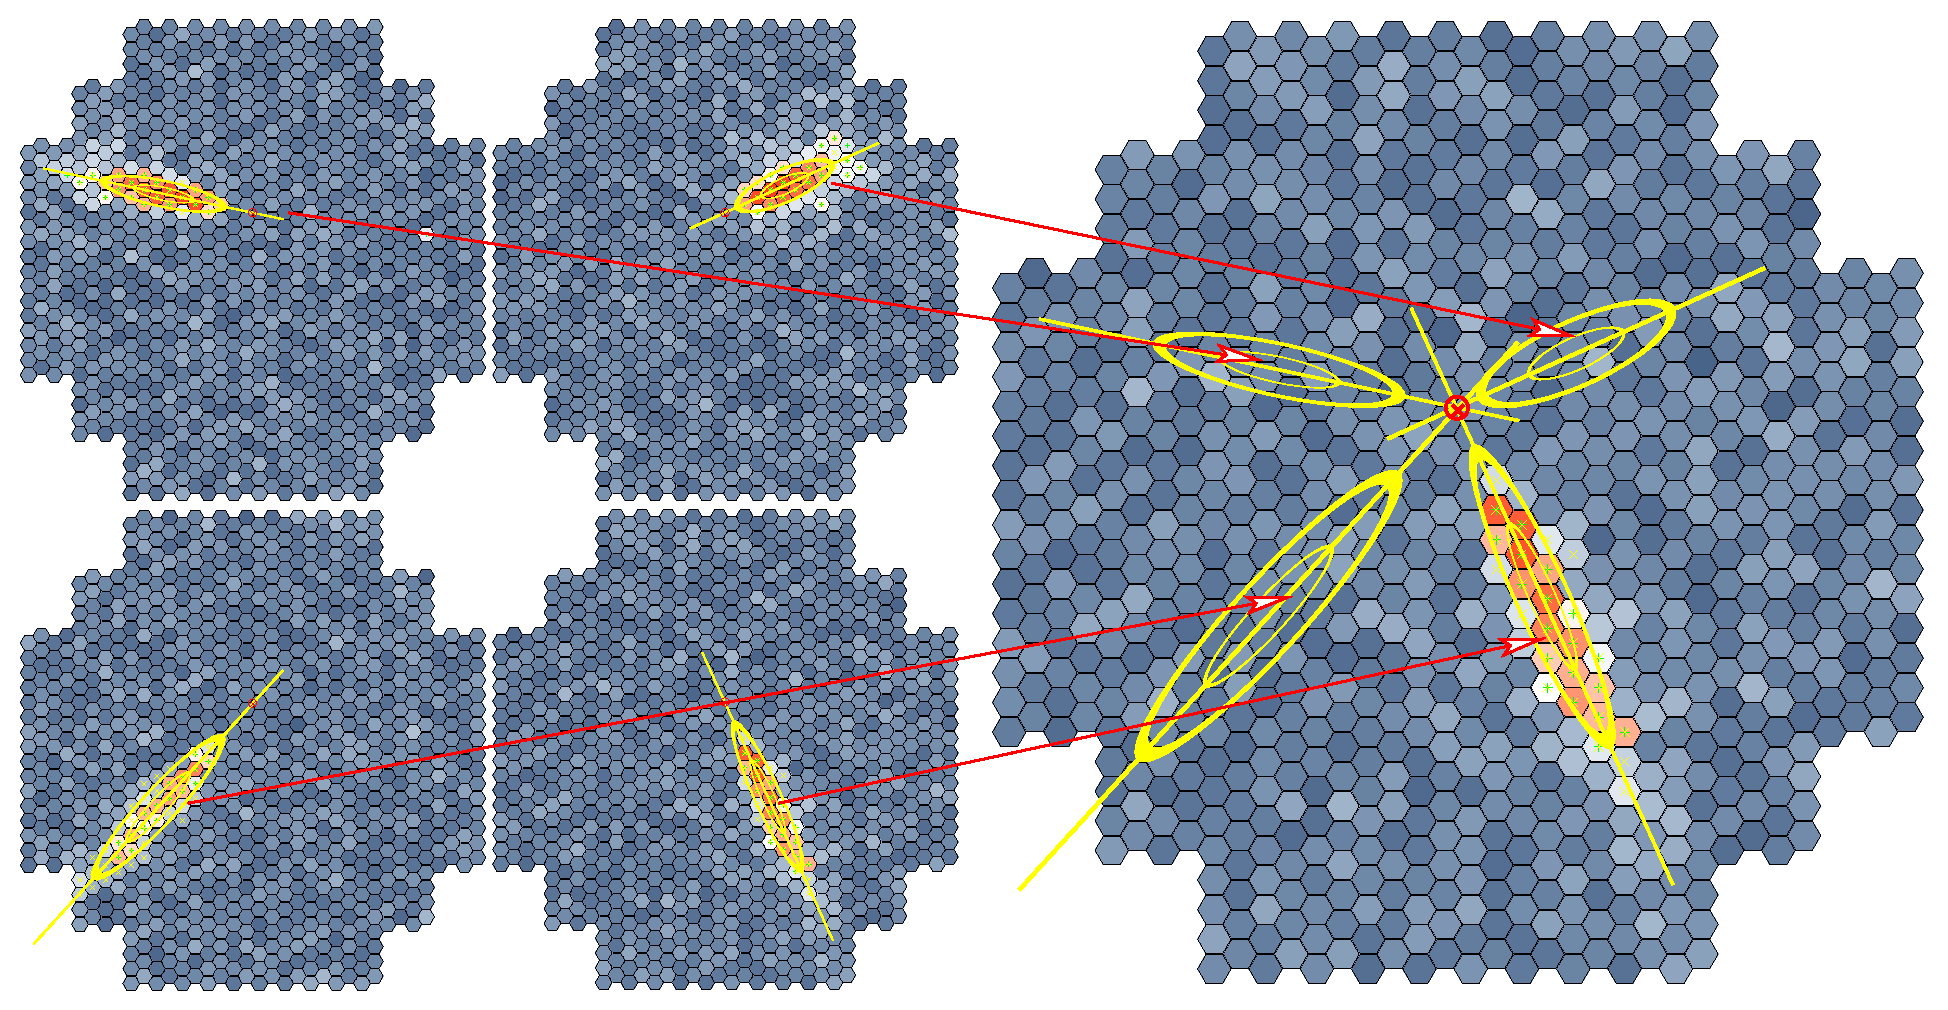
\includegraphics[width=0.96\linewidth]{images/Stereo}
  \caption[Gamma-ray EAS at a telescope array.]{Gamma-ray induced air shower incident at a telescope array (left). Image of an air shower on the camera plane. Each telescope image is characterized by an ellipse (right).}
  \label{fig:camera_face}
\end{figure}

Modern IACTs use multiple telescopes operating in conjunction, which increases effective area as well as directional resolution. Combining the images from the different telescopes enables stereoscopic imaging allowing for reconstructing the axis of the air shower as shown in Fig. \ref{fig:IACT}. The majority of EAS are generated by high energy cosmic rays, composed primarily of protons and nuclei, rather than gamma rays. The dominant interactions of these protons -- nuclear hadronic interactions -- are the same process commonly seen in particle colliders, producing showers dominated by high energy $\pi$ mesons ($\pi^0$, $\pi^\pm$).
\subsection{The VERITAS Instrument}
The VERITAS instrument consists of four telescopes, each consisting of a reflector, a camera box, and a counterweight. The reflectors on each telescope are 12 m diameter spherical Davies-Cotton mirrors \cite{DaviesCotton}. The four telescopes are arranged in order to maximize collection area while being close enough for multiple telescopes to fall within the light pool for an air shower. Having multiple telescopes within the light pool allows for better stereoscopic reconstruction as demonstrated in Fig. \ref{fig:camera_face}. The distance between adjacent telescopes is $\sim 100$ m and the radius of the light pool for energies $>100$ GeV is $\sim 130$ m.\par

Each VERITAS telescope uses 345 identical hexagonal spherical mirrors (of area 0.322 m$^2$ and radius-of-curvature of approximately 24m) giving a total reflector area of nearly $110$ m$^2$. The hexagonal shape allows for more efficient packing of mirrors on the reflector surface.\par
The individual hexagonal mirrors need to be manually aligned so that the entire reflector will act as a single dish. The measure of the alignment of these mirrors is the point spread function (PSF), which describes the response of the detector to a point source at infinity. The better aligned the system, the smaller the value of the resulting PSF.\par
% FIX ALL OF THIS PLAGIARISM
\begin{figure}[htbp]
  \centering
  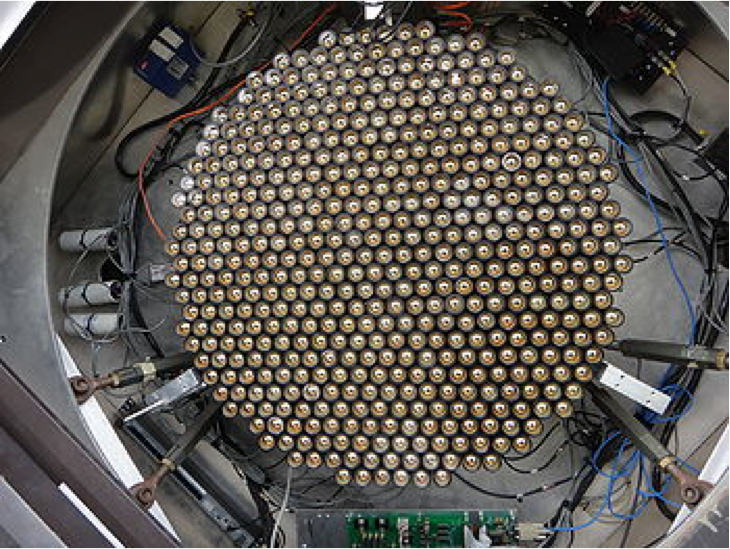
\includegraphics[width=0.58\linewidth]{images/Camera_PMT}
  \caption[PMTs in the VERITAS camera.]{The PMT ``pixels'' in the VERITAS Camera. Picture taken from \cite{Kieda:2013wom}}
  \label{fig:VERITAS_Cam}
\end{figure}
The camera in a VERITAS telescope is located at the focal plane of the telescope (12 meters from the mirrors) in a ``focus box" of dimension 1.8m x 1.8m. The camera consists of 499 closed-packed circular photomultiplier tubes (PMTs, see Fig. \ref{fig:VERITAS_Cam}), giving an angular pixel spacing of 0.15 degree and a total field-of-view (FOV) of 3.5 degrees. The PMTs are arranged in a hexagonal pattern to maximize coverage.\par

At the low end of the VERITAS energy range, fluctuations in the night sky background (NSB) and (single) muons from cosmic-ray showers constitute a large fraction of the observed single-telescope events. VERITAS employs a three-tier trigger system to reduce the rate of these background events. The first trigger system works on the single-pixel level, the second checks for specific patterns of single level pixels within a timing window, and the third works at the array level, requiring simultaneous observations of an air-shower event in multiple telescopes (ensuring a "stereoscopic" view of the event). The three trigger levels are designated L1, L2 and L3.\par

% L1 Trigger system
The L1 trigger, which is the pixel-level trigger system, has constant fraction discriminators (CFDs) and threshold discriminators for each PMT in the telescope cameras. This trigger requires the signal from a PMT channel to be above a particular threshold, reducing contamination from the night sky background and electronic noise. This information is then passed on to the L2 trigger.

% L2 Trigger system
The L2 trigger, reduces effects from NSB and electronic noise by requiring correlations between adjacent pixels. Specifically, this trigger only triggers an output pulse when several adjacent pixels surpass the L1 discriminator threshold within some coincidence window (about 6 ns). The L3 trigger uses this to determine whether to store the data.

% L3 Trigger system
Relativistic muons in the atmosphere radiate Cherenkov radiation and comprise a large background source for Cherenkov telescopes at low energies. Muons decaying close to a telescope face produce rings in the camera, but these rings will only be large enough for detection by a single telescope. With this in mind, the L3 trigger is an array-level trigger which depends on receiving telescope level triggers from more than one telescope. Effective removal of the muon background allows sensitivity to the lower energy range where these backgrounds would otherwise dominate.
\section{Shower Image Parameters}
\label{shower-img-params}
The shower image parameters are the input to the direction reconstruction that is the focus of this work. In any given telescope, the shower image is parameterized using various measurements including
\begin{itemize}
\item the image axis -- defined as the line minimizing the signal-weighted sum of squares of perpendicular distance between triggering pixels (see \ref{fig:image_axis}).
\item the time gradient -- a measure of the difference in time of arrival, along the image axis, of the signal at a pixel (see \ref{fig:time_gradient}).
\item the length of the image (see \ref{fig:hillas_ellipse}) -- the r.m.s spread of the signal-weighted triggered pixels parallel to the image axis \cite{Hillas:1985}.
\item the width of the image (see \ref{fig:hillas_ellipse}) -- the r.m.s spread of teh signal-weighted triggered pixels perpendicular to the image axis. The length and width together provide the major and minor axis of an ellipse containing the majority of the signal, and are referred to as the Hillas parameters and the Hillas ellipse.
\end{itemize}
A number of other parameters are used in the complete reconstruction of the shower, but these are the most relevant to the direction reconstruction, and specifically to the direction reconstruction process using the boosted decision tree (BDT) angular reconstruction.
\begin{figure}[htbp]
  \centering
    \subfigure[Image axis parameter for a shower]{ 
      
\includegraphics[width=0.45\linewidth]{images/placeholder}
      \label{fig:image_axis}
    }  
    \subfigure[Time gradient parameter for a shower]{ 
      
\includegraphics[width=0.45\linewidth]{images/placeholder}
      \label{fig:time_gradient}
    }
  \caption[Image parameters]{Image Parameters}
  \label{fig:img_params}
\end{figure}

\subsection{The \disp Parameter}
The \disp parameter is a measure of the displacement between the center of the Hillas ellipse (the center of gravity of a shower image at a telescope), and the origin of the shower in the camera plane (Fig. \ref{fig:Disp_FOV}). This is a telescope-level parameter with a head-tail ambiguity, but with multiple telescope images, it can be used in estimating the direction of the initiating gamma ray. This is based on the idea in method (c) described in Hofmann\cite{Hofmann:1999dx}.
\begin{figure}[htbp]
  \centering
  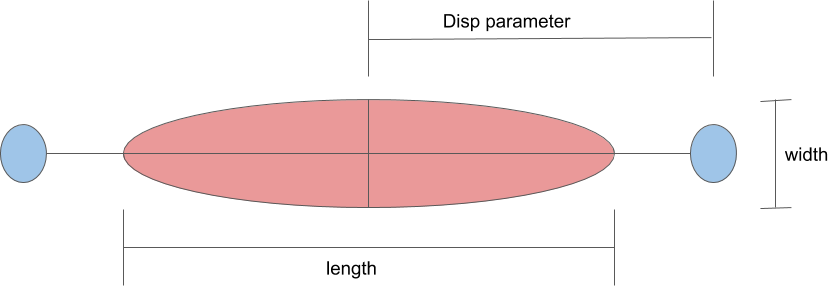
\includegraphics[width=.58\linewidth]{images/Disp_param}
  \caption[The Hillas ellipse]{Hillas Ellipse (red), with the major axes and the estimated or calculated location of the origin of the shower in the camera plane (blue).}
  \label{fig:hillas_ellipse}
\end{figure}

\begin{figure}[H]
  \begin{center}
      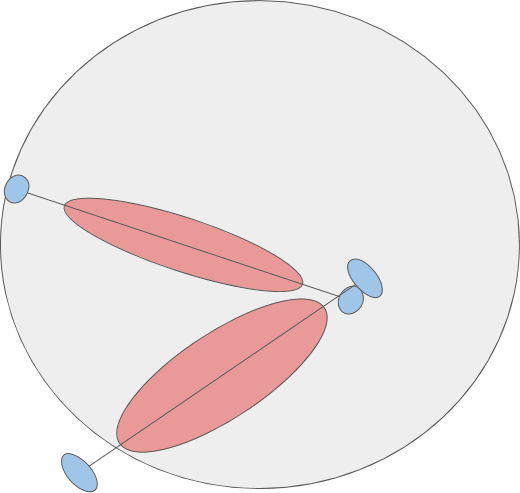
\includegraphics[width=0.48\linewidth]{images/Disp_FOV}
      \label{fig:Disp_FOV}
  \end{center}
  \caption[The Disp Parameter]{The Hillas ellipses (see Fig. \ref{fig:hillas_ellipse}), as used to reconstruct shower direction. In a single telescope image, there is an ambiguity in the direction of the displacement from the center of gravity of the image. However, in a multi-telescope array this ambiguity can be resolved by looking at several Hillas ellipses in conjunction and minimizing the location of the shower source.}
  \label{fig:Disp_FOV}
\end{figure}

% \footnote{As of VEGAS 2.5.4, method5t uses disp=f(zenith, mean scaled width, mean scaled height, size, azimuth, loss, time gradient), where loss is the shower image outside of the Hillas ellipse.}

\end{document} 